\chapter{Исследовательский раздел}
\label{cha:research}

В данном разделе приведено сравнение алгоритмов по времени работы.
Все параметры замерялись на устройстве со следующими техническими характеристиками:
\begin{itemize}
	\item операционная система macOS Monterey 12.6 \cite{monterey};
	\item оперативная память 16 Гб;
	\item процессор 2,3 ГГц 8‑ядерный Intel Core i9 9 поколения \cite{intel};
	\item 8 физических ядер, 16 логических ядер \cite{intel}.
\end{itemize}

Во время замеров ноутбук был подключен к сети питания и нагружен только приложениями, использующимися при замерах.

\section{Демонстрация работы программы}

На рисунке \ref{img:example} представлен пример работы программы.

\begin{figure}[ph!]
	\center{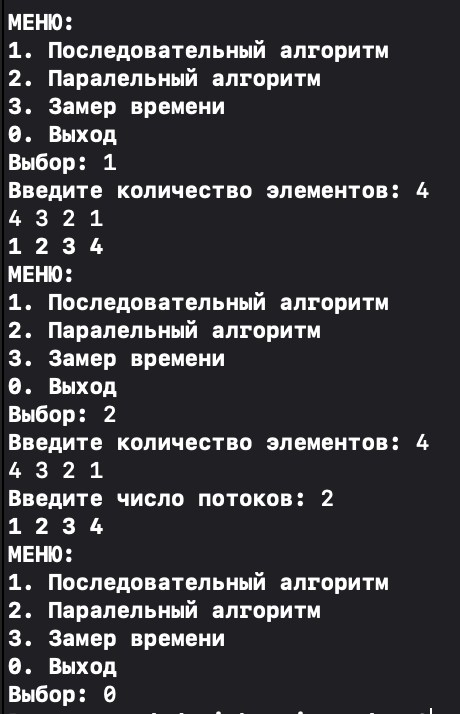
\includegraphics[scale=1.0]{img/example.png}}
	\caption{Пример работы программы}
	\label{img:example}
\end{figure}

\section{Измерение времени работы реализаций алгоритмов}

Процессорное время замерялось при помощи функции time из заголовочного файла time.h~\cite{cplusplus}. Результаты сформированы в виде графиков при помощи библиотеки matplotlib~\cite{matplotlib}.  Каждый алгоритм был выполнен 30 раз, а затем время усреднялось.
Время было замерено на случайно сформированных массивах.

На рисунках \ref{fig:timings_fixed_size} -- \ref{fig:timings_fixed_threads} на осях X указано количество элементов во входном массиве. Время на осях Y указано в секундах.

\begin{figure}[ph!]
	\center{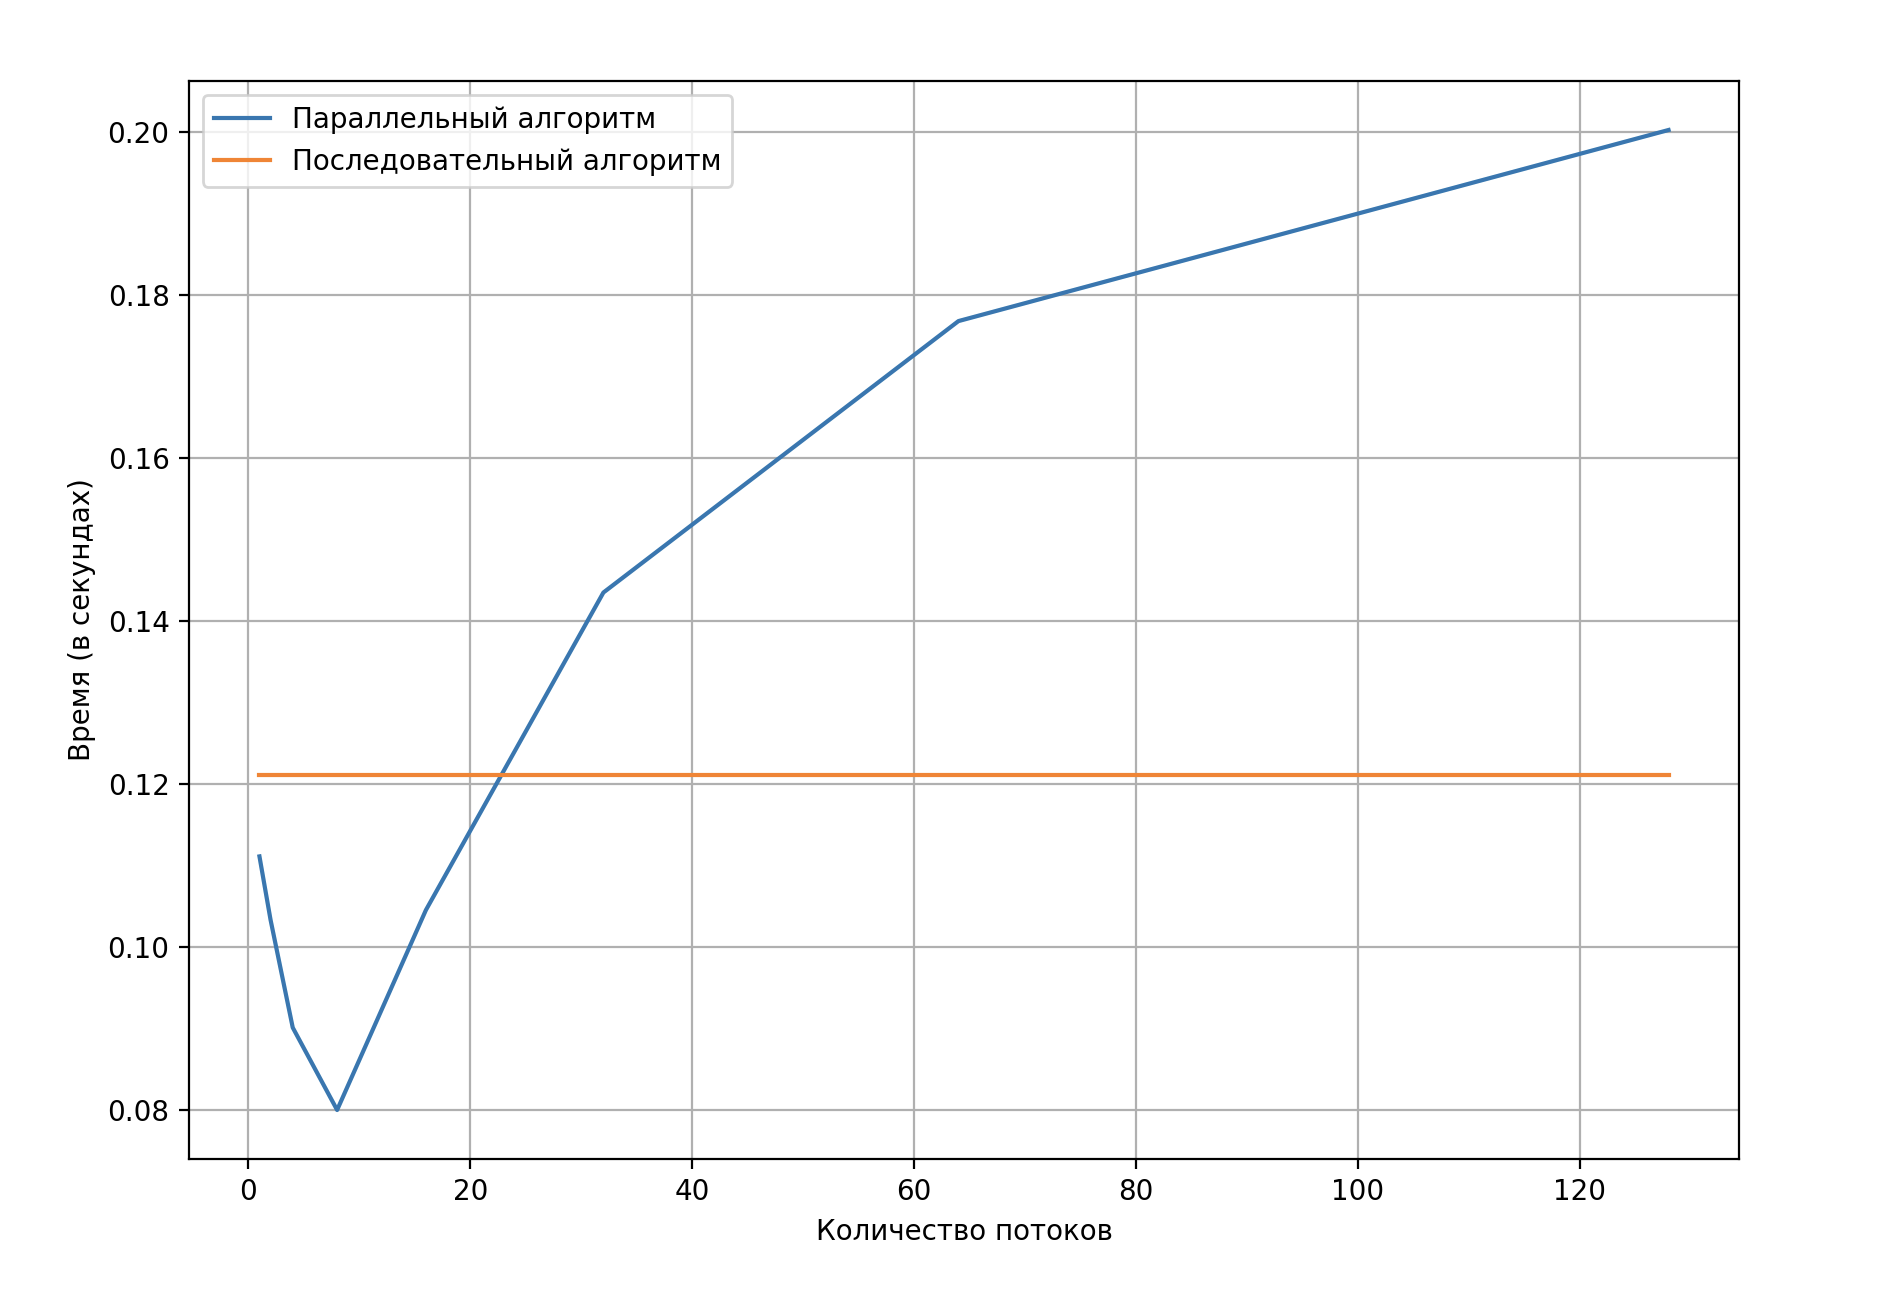
\includegraphics[scale=0.5]{img/timings_fixed_size.png}}
	\caption{Результаты замеров времени реализаций алгоритма битонной сортировки для разного количества потоков (количество элементов в массиве равно 1024)}
	\label{fig:timings_fixed_size}
\end{figure}

\begin{figure}[ph!]
	\center{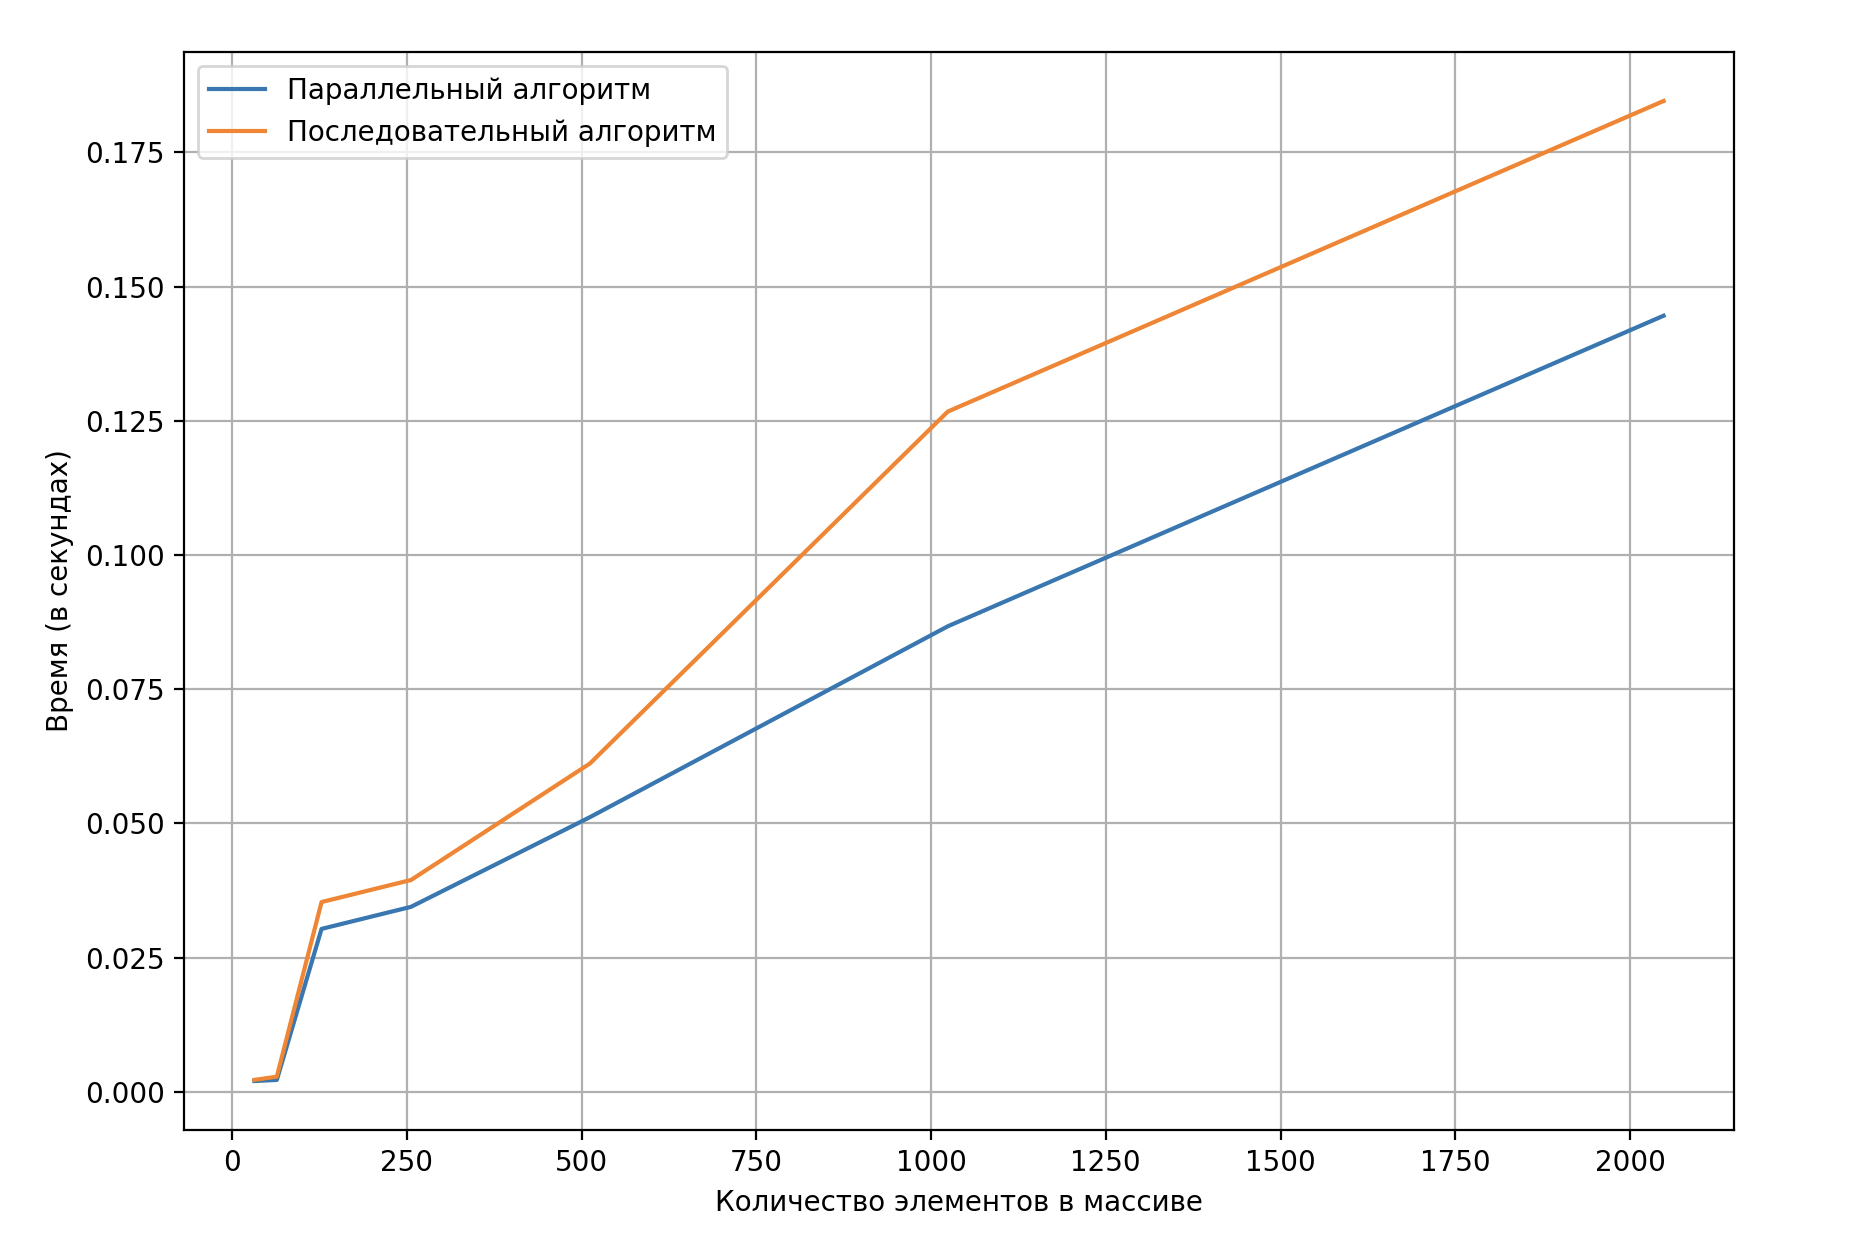
\includegraphics[scale=0.55]{img/timings_1_thread.png}}
	\caption{Результаты замеров времени реализаций алгоритма битонной сортировки для 1 потока}
	\label{fig:timings_1_thread}
\end{figure}

\begin{figure}[ph!]
	\center{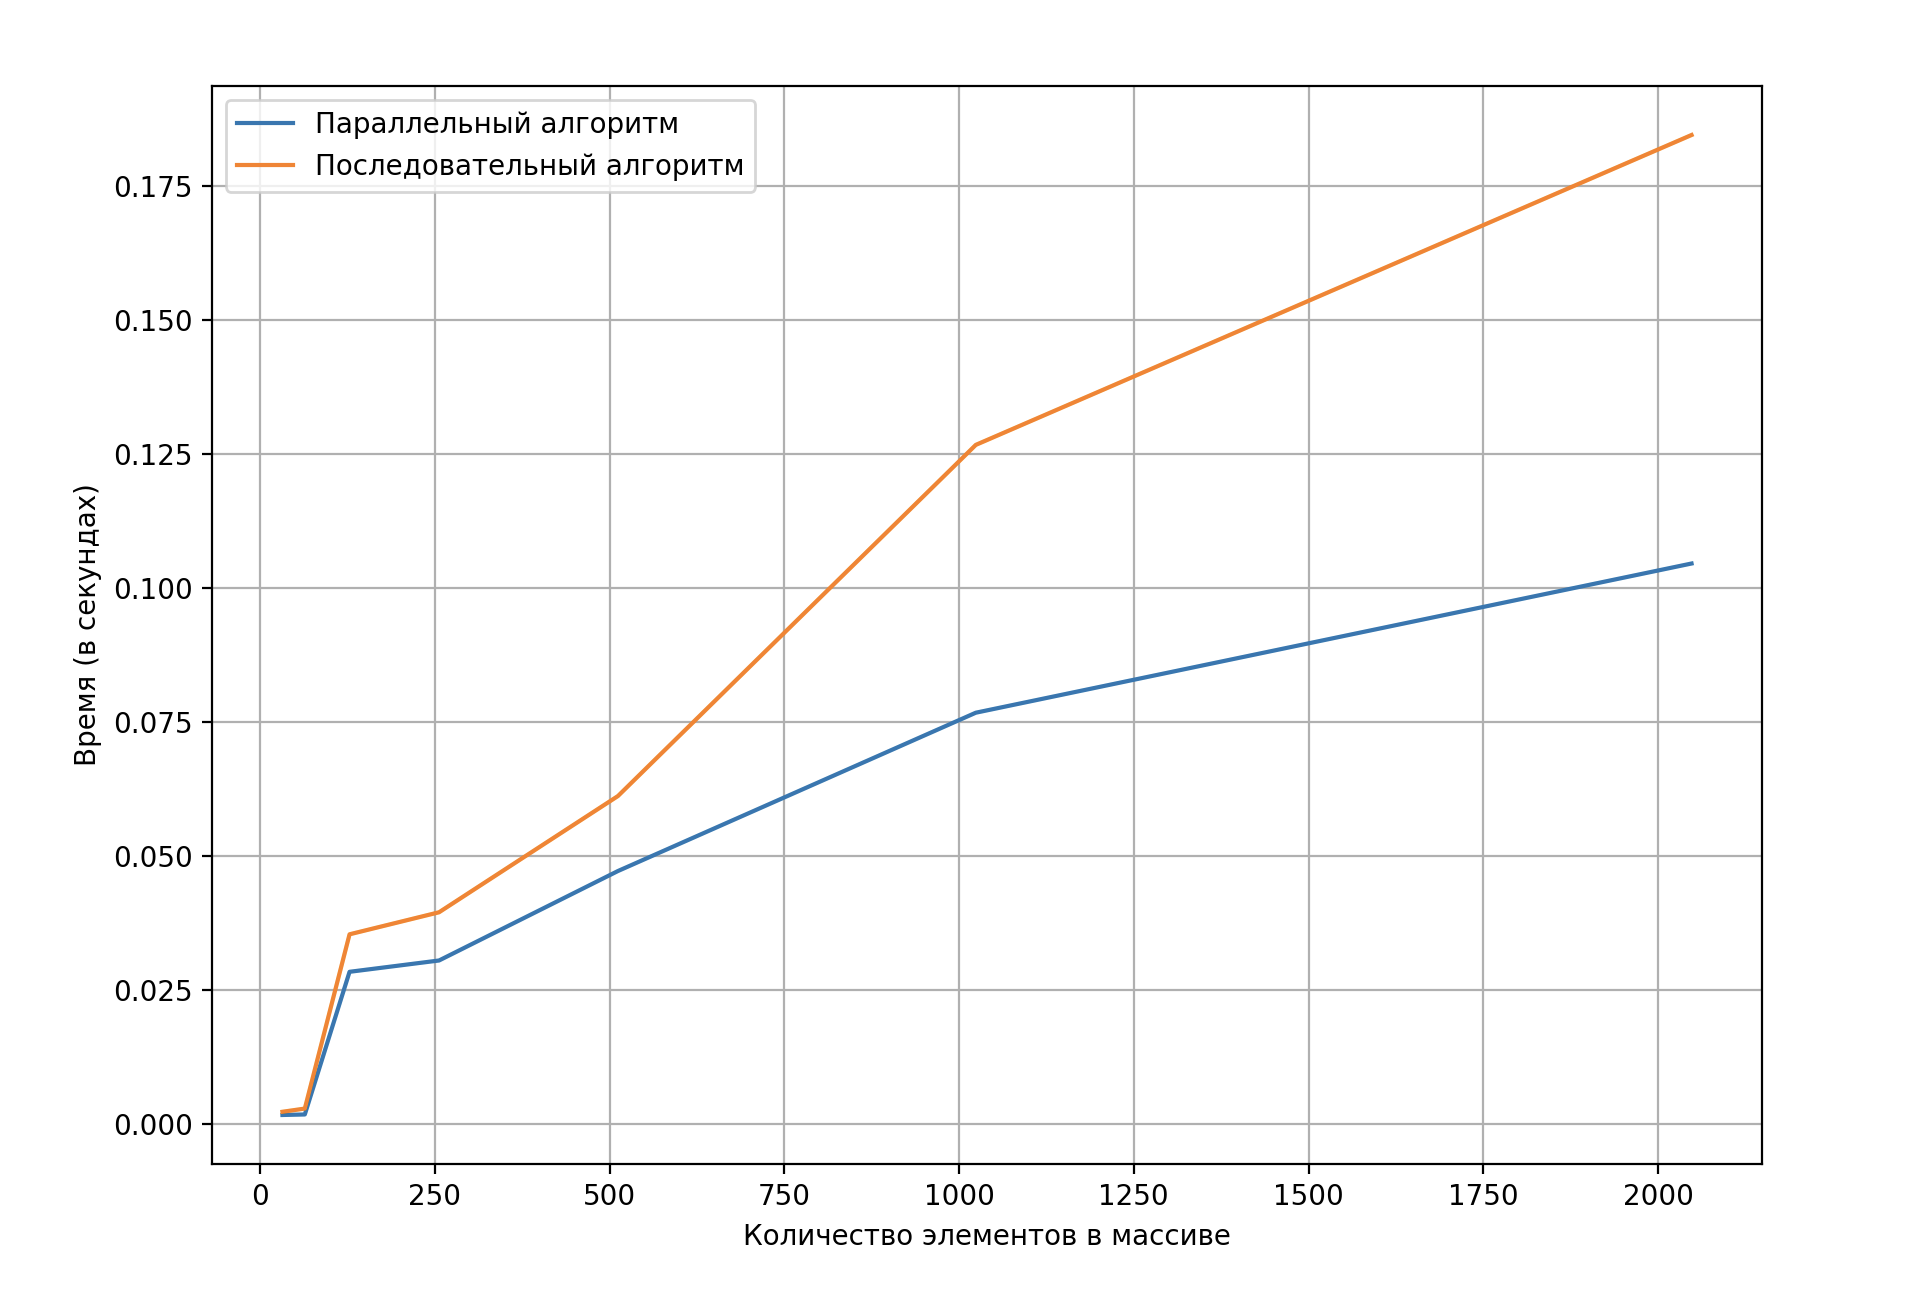
\includegraphics[scale=0.55]{img/timings_8_threads.png}}
	\caption{Результаты замеров времени реализаций алгоритма битонной сортировки для 8 потоков}
	\label{fig:timings_fixed_threads}
\end{figure}

\clearpage

\section*{Вывод}

В результате эксперимента можно сделать вывод, что при использовании 8 потоков, многопоточная реализация алгоритма битонной сортировки лучше реализации без многопоточности в среднем на 35\% при количестве элементов в массиве равном 1024. 


